Telecommunications networks depend increasingly on optical components to increase data speed while minimising energy consumption. But photonics still has much unfulfilled potential. \\
\\
The density of transistors in computers has successively followed Moore's law for the past decades, with the consequences of continuously increasing processing speed, but also the number of signal-carrying cables and signal-processing devices. While optical fibres are well-used for long-distance communication, short-distance communication within e.g. computer clusters commonly rely on electrical signals and devices.\\
\\
Optical fibres are used to send signals at light speed with low heat production over large distances at an affordable price. Wavelength-division (de-)multiplexers are used to either split or combine these optical signals, making them a valuable tool in signal processing, especially for short-distance communication. But current wavelength demultiplexers have fairly large footprints, such as IBM's 1-to-8 wavelength (de-)multiplexer \cite{IBMdemultiplexer}, which measures 500 $\times$ 200 \si{\micro m^2}. \\
\\
In this project, we wish to create a 1-to-2 wavelength demultiplexer with a 2.8 $\times$ 2.8 \si{\micro m^2} footprint, more than 12000 times smaller than the (de-)multiplexer from IBM. The demultiplexer must split wavelengths of 1300 nm and 1550 nm into two separate output waveguides. A device with the same goals was previously created at Stanford\cite{Stanford} with an inverse design strategy not relying on topology optimisation. We wish to show that topology optimisation will yield better results in terms of decoupling the signal, as well as improving the insertion loss.\\
\\
The software used in this project was developed by research groups at DTU Photonics and DTU Mechanics. The software simulates transmission of light through a silicon structure, and finds a local solution for the design, given specified objectives and an initial structure. The design goal is achieved through topology optimisation; An inverse design-method relying on Finite-Difference Time-Domain (FDTD) calculations where the silicon structure is iteratively regulated with respect to a specified set of objective functions.

\begin{figure}[h!]
    \centering
    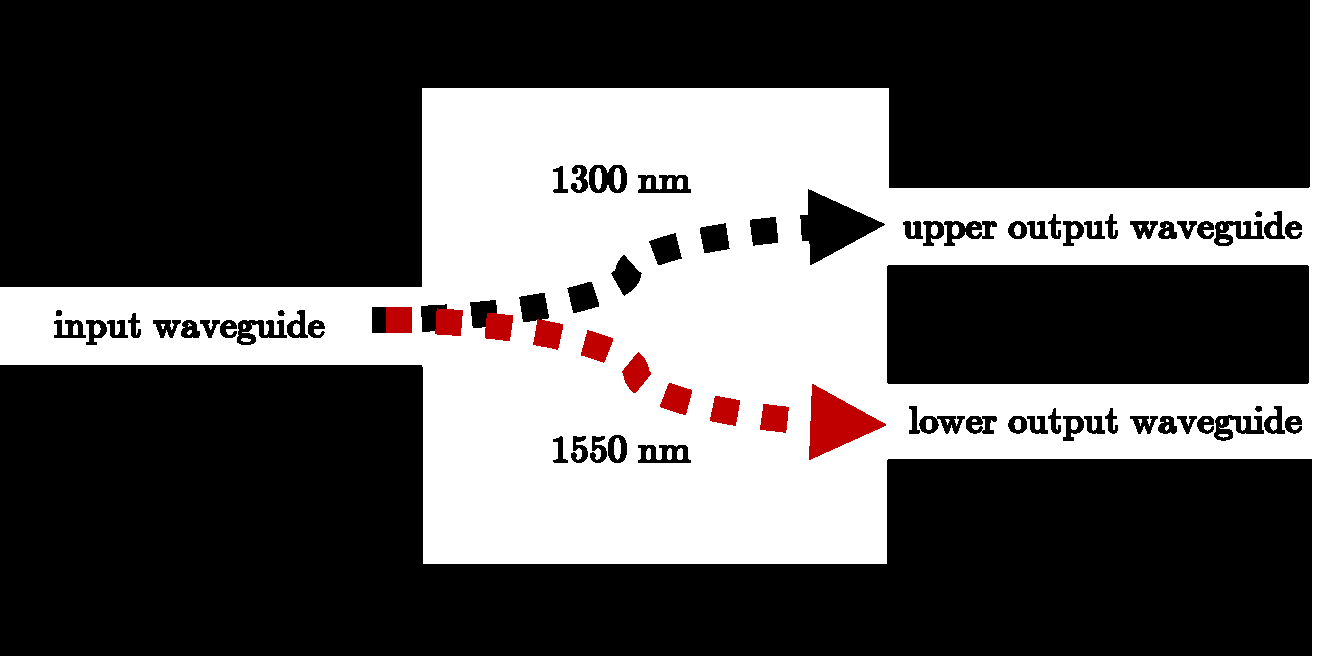
\includegraphics[width=0.7\textwidth]
    {fig/introduction/demultiplexer.pdf}
    \caption{The goal of this project: Creating a wavelength demultiplexer, a device for splitting optical signals, through topology optimisation.}
    \label{fig:my_label}
\end{figure}
